% vim: set fenc=utf-8 ft=latex encoding=utf-8
% -*- mode: latex; coding: UTF-8; -*-

\newif\ifdraft
\drafttrue

\ifdraft
	\documentclass[conference, draftclsnofoot]{IEEEtran}
	\def\baselinestretch{1}
	\setlength{\marginparwidth}{2cm}
\else
	\documentclass[conferece, final]{IEEEtran}
\fi

\usepackage[T1]{fontenc}
\usepackage[utf8]{inputenc}

\newcommand{\TheTitle}{Visualizing Release Information of Linux}
\newcommand{\TheAuthors}{Evan Wilde}
\newcommand{\TheEmails}{etcwilde@uvic.ca}
\newcommand{\TheSubject}{Digesting large amounts of commit data}
\newcommand{\TheKeywords}{Linux, git, data structures, tree data structures}

\synctex=1

\usepackage[hyphens]{url}
\urlstyle{same}

\ifdraft
	\usepackage[unicode=true,bookmarks=false,breaklinks=false,
		pdfborder={0 0 0},backref=none,colorlinks=true]{hyperref}

\else
	\usepackage[unicode=true,bookmarks=false,breaklinks=false,
		pdfborder={0 0 0},backref=none,colorlinks=false]{hyperref}
\fi

\usepackage[nospace]{cite}

% Table Support
\usepackage{dcolumn}
\usepackage{longtable}

\usepackage{balance}
\usepackage{placeins}
\usepackage{multirow}

% Extra support
\usepackage{xspace}
\usepackage{caption}

% Fix any bad-hyphenations here
\hyphenation{}

% \ifdraft
%     \usepackage[colorinlistoftodos]{todonotes}
%     \newcommand{\evan}[1]{{\color{blue}\emph{Evan Says: #1}}\xspace}
%     \newcommand{\evantodo}[1]{{\color{blue}\emph{Evan Todo: #1}}\xspace}
%     \newcommand{\dmg}[1]{{\color{blue}\emph{dmg Says: #1}}\xspace}
%     \newcommand{\dmgtodo}[1]{{\color{blue}\emph{dmg Todo: #1}}\xspace}
% \else
%     \usepackage[disable]{todonotes}
%     \newcommand{\evan}[1]{}
%     \newcommand{\evantodo}[1]{}
%     \newcommand{\dmg}[1]{}
%     \newcommand{\dmgtodo}[1]{}
% \fi
    \usepackage[colorinlistoftodos]{todonotes}

\newcommand{\tool}{{\emph Linvis}\xspace}


    \newcommand{\evan}[1]{{\color{blue}\emph{Evan Says: #1}}\xspace}
    \newcommand{\evantodo}[1]{{\color{blue}\emph{Evan Todo: #1}}\xspace}
    \newcommand{\dmg}[1]{{\color{blue}\emph{dmg Says: #1}}\xspace}
    \newcommand{\dmgtodo}[1]{{\color{blue}\emph{dmg Todo: #1}}\xspace}


%%% Local Variables:
%%% mode: plain-tex
%%% TeX-master: t
%%% End:


\begin{document}

\title{\TheTitle}
\author{
\IEEEauthorblockA{\TheAuthors}
\IEEEauthorblockN{Department of Computer Science,
                    University of Victoria, Canada.}
\IEEEauthorblockA{Email: \TheEmails}
}
\maketitle
\begin{abstract}

	With an average of over 900 top-level merges into the Linux kernel per
	release, some containing thousands of commits, many containing hundreds
	of commits, maintenance of older versions of the kernel becomes nearly
	impossible. For security, performance, and changing hardware,
	maintainers must understand the changes made to current versions of the
	kernel, and show these changes fit into older versions in order to make
	the necessary merges and modifications to the older versions. Current
	tools provide information about repositories through the directed
	acyclic graph (DAG) which is helpful for smaller projects, but with the
	scale and number of branches in the kernel, the DAG becomes
	overwhelming very quickly.

	In this paper, we present a tool that uses the dataset collected by
	German et al. to build a tool that uses a vine model instead of the
	DAG. This tool is designed to cater to the needs of users looking for a
	top-down approach, or a bottom-up approach to navigating the commit
	information of the kernel.
\end{abstract}

\begin{IEEEkeywords}
\TheKeywords
\end{IEEEkeywords}

\section{Introduction}

Maintainers of older version of the Linux kernel must sift through thousands of
commits with tools that are unable to filter and effectively visualize projects
that are of the scale of the kernel. Tools like Gitk provide users with the
full view of the DAG, showing all merges and commits. For smaller projects,
this information is useful for showing the relation between various branches.
With large modular projects, like the Linux Kernel, the DAG becomes a tangled
mess (\ref{fig:gitk}) of commits, merges, and the links between them, making it
difficult to derive an explanation of the changes.  Github provides a DAG view
for most projects, but is unable to display the DAG of projects as large as the
Linux Kernel.

\begin{figure}
	\centering
	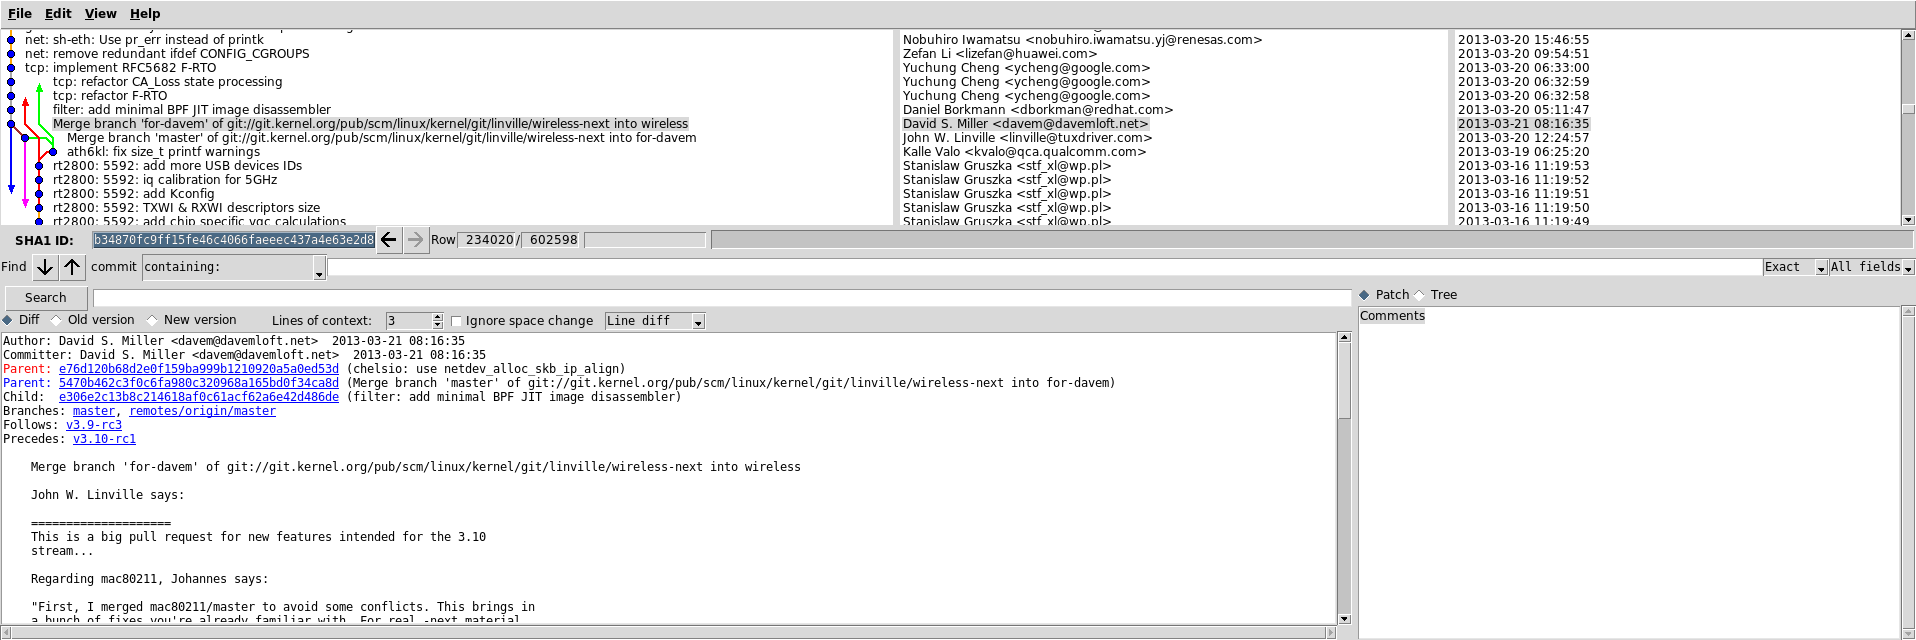
\includegraphics[width=0.47\textwidth]{figures/gitk.png}
	\caption{DAG view in Gitk}
	\label{fig:gitk}
\end{figure}

Git log, Gitk, and other similar tools only store the authored date of a
commit. A commit may be merged into the project at any time, regardless of when
the commit was authored. Because of this, performing date-range queries does
not provide meaningful results. Performing a date-range query using other tools
over the span of a release will contain results that are for previous versions
of the kernel, and may not contain all of the results for that kernel if
patches were merged after the release date.

German et al. recorded the metadata of every commit and merge in the Linux git
repository from 2012 to 2015, including data that is not stored by git. We are
able to use this information to generate sets of trees instead of a DAG. The
root of each tree is the top-level merge performed by Linus, which merges a
given commit into the kernel.

In this paper, we present the design decisions behind a web-based tool built
around a tree-based model instead of the DAG. We demonstrate the advantages of
this model over the use of the DAG. Our tool provides information about the
location of a given commit in the respective merge tree, the files edited, the
modules edited, and the commit message in a given commit or merge. The tool
allows users to apply various filters, including the release, a keyword or
phrase from the log preview, the name of the author, or the commit id. The user
can request all the top-level merges containing a commit or merge that matches
the query, or all commits and merges that match the query.

Our core model provides many advantages to other tools. Breaking the data by
merge tree removes the commits and merges of other components of the kernel
from the visualization, providing a clearer picture of what is happening in a
given merge. This model provides additional support to edited file information.

All top-level merges to a given version of the kernel are merged between the
start and release date. Our tree construction allows us to use the top-level
merges to find all merges and commits that have an effect on a given version of
the kernel. The model allows us to better provide mechanisms for performing
date-range queries, providing access to all commits that have an effect on a
given release, even if the commit comes before the start date, or the release
date.

\section{Related Work}

\subsection{Gitk}
Gitk, Gitg, and other similar git repository visualizing tools use the DAG as
the central organization. For smaller projects, this model is sufficient for
providing meaningful information, but in larger projects like the Linux kernel,
the branches become too tangled and too deep to derive any meaning from the
DAG. The DAG model allows users to go to the next commit in the chain, go to
the previous commit in the chain, or jump to the parent merge. This suggest
that Gitk and similar tools are designed for users working with a bottom-to-top
approach. With this model, it is difficult for users to see what other commits
are involved with a given merge. Gitk only provides file information on
commits, as it is unable to quickly find all files edited by a merge. It is up
to the user to remember what files were edited in each of the commits involved
in a given merge. In some of the larger merges, some containing over 1500
edited files, this task become nearly impossible.
% cid: 73287a43cc79ca06629a88d1a199cd283f42456a, 1800 commits, 1500 files
Other DAG visualization systems, like the GitHub viewer (\ref{fig:gitfail}),
are unable to provide a visualization for projects that are as large as the
kernel.

\begin{figure}[h!]
	\centering
	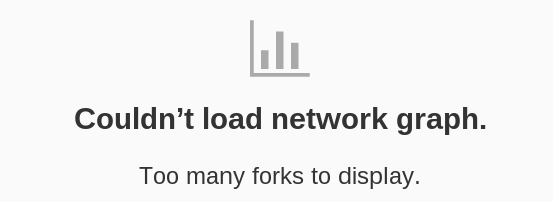
\includegraphics[width=0.45\textwidth]{figures/github_viewer.png}
	\caption{Github Failure Message}
	\label{fig:gitfail}
\end{figure}

%% Check for papers if they exist
%% This tool isn't specifically designed for showing Linux

\subsection{Treemap visualizer}
University of Maryland presented a treemap design (\ref{fig:treemap}) for
displaying all the file structure of a given version. Treemaps are good for
displaying the topology of shallow, wide trees, making it a good candidate for
displaying file systems. Treemaps are limited in what information can be
displayed. The information within the treemap does not provide clear insight on
what changes were made to the files in the given release. The treemap
visualization only provides information on where the file is located within the
filesystem. File systems and the merge tree of the kernel share many
similarities, in both cases, the representative trees are wide and shallow,
suggesting that a treemap could potentially work to visualize the commit and
merge structure of the kernel.

The treemap is unable to take into account multiple merges at the same level
with the same name. There is an additional dimension, in that the commits and
merges are ordered in time. The treemap design is unable to show the ordering
of the merges and commits.

The treemap design is also designed for working with data of differing types.
In the filesystem, there are many kinds of files.  There are text files,
scripts, images, binary files, and other types. These can be given colours
making differences stand out. There is no obvious way to assign meaningful
types to the commits such that all the commits within a given merge do not all
have the same colour.

Finally, the treemap does not provide any additional information about the
contents of each cell, only that the cell exists. The user is unable to see
their current position within the map, or if we assume that their current
position is the larges surrounding box, they can no-longer see how their
current position interacts with the rest of the system.
%% https://www.cs.umd.edu/hcil/millionvis/Treemap_Visualization_of_the_Linux_Kernel_2_5_33.html
%% Find paper for this maybe?

\begin{figure}[h!]
	\centering
	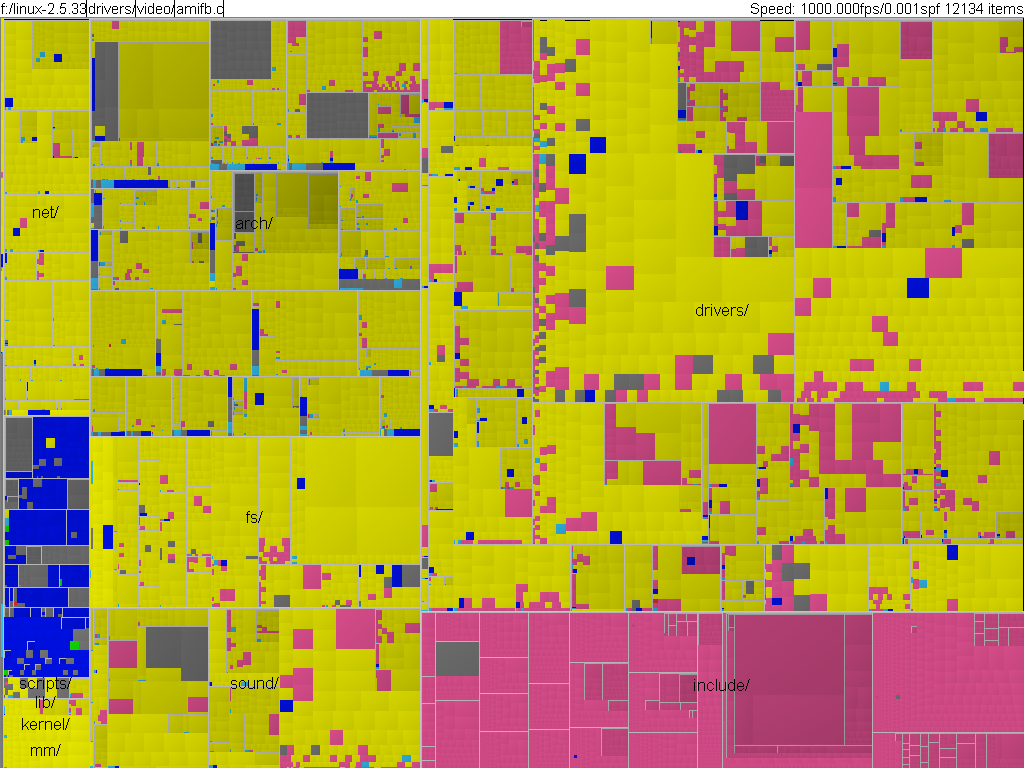
\includegraphics[width=0.47\textwidth]{figures/kernel-files.png}
	\caption{Treemap of Linux 2.5.33 file structure}
	\label{fig:treemap}
\end{figure}


\subsection{List viewer}
Moghaddam designed a web-based visualization tool displaying the chain of
merges into the kernel. There is no information on what commits are within a
given merge, or what files were edited. The visualization tool provides
information about who authored the commit and when it was authored.
\evantodo{Link to tool}
%% http://web.uvic.ca/~arasbm/gitVisualizations/linuxRGraph.html
%% Find paper for this maybe?

\begin{figure}[h!]
	\centering
	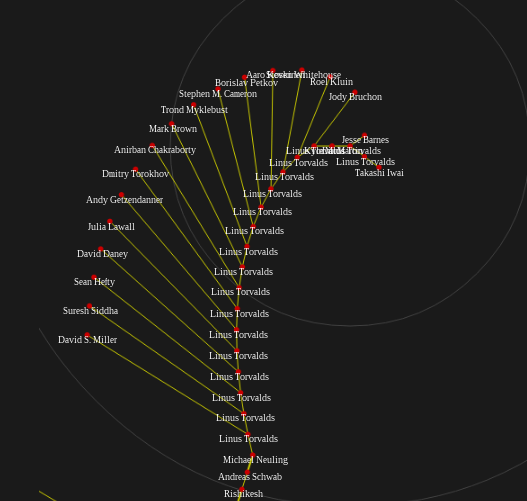
\includegraphics[width=0.47\textwidth]{figures/gitvis.png}
	\caption{List Viewer}
	\label{fig:listviewer}
\end{figure}


\section{Core Model}
Each merge may contain zero or more children of other merges or commits.
Commits have no children, and therefore are always leaf nodes, but commits
contain information about what files are edited, how many lines are edited, and
other important information.

Core Model:
	Merges are inner nodes
	Commits are leaf nodes

\section{Implementation Details}

We built a we-based tool to provide information about the kernel.
We chose to use Nginx as the main web server, postgresql as the dbms, and Flask
as the framework for generating the dynamic content.

Nginx is a high-performance, scalable HTTP and mail server. Started in 2002,
the project is much younger than the Apache project, and designed with massive
scalability and multi-processing in mind. Instead of using request-driven
threading, Nginx uses an event-driven architecture, making it more scalable,
proving itself as being the web server behind Netflix, Hulu, GitHub, Tumblr,
and many other popular sites.

Postgresql is our dbms of choice, providing fast and reliable results. There
are multiple reasons behind choosing postgresql over another dbms. The main
reason being that the dataset provided from \evantodo{paper} was generated from
a postgresql database, allowing us to import the data directly without any
further conversions. The secondary reason is that we are more familiar with
postgresql than the other systems available.

We chose the python micro-framework Flask for generating the dynamic content.
Working with flask is simple and easy.

The database itself is broken down into 5 main tables; commits, filesmod, logs,
pathtomerge, and releases. Commits contains most of the metadata for each
commit, it contains the author, the authored date, and committer, the commit
date, a boolean saying what is a merge, and the diff. Filesmod contains the
information on what files were modified for the commits. Since a file may be
modified by multiple commits, and a commit may be modifying multiple files, we
can do one of two things for the primary key. We could use both the filename
and the commit id as the primary key, but we just use an index. The filesmod
table contains the filename, the commit id, the number of lines added, and the
number of lines removed. Trivially, it contains the index, but that isn't
necessary for anything beyond the primary key. Logs contains the information
for each commit log, this is the one-liner preview message and the full
message. Pathtomerge is the important table. Pathtomerge contains the commit
id, the number of merges between the commit and the top-level merge with the
kernel, the next merge in the merge path up to the top-level merge with the
kernel, the top-level merge into the kernel, and when it get merged into the
kernel. The information in this table must be generated periodically by the
server because we are unable to generate the tree structure correctly straight
from the information stored by git. Pathtomerge does not contain any top-level
merges, as these will never have a next merge in the tree, since we are only
storing the parents and not the children, storing the top-level merge is
redundant and unnecessary. The releases table stores the release information.
It contains the version name, whether the version is a candidate release or a
real release, the previous version, the previous non-candidate release version
the previous version commit id, the previous non-candidate release version
commit id, and the commit id of this version. The version commit id represents
the last top-level merge into the version of the kernel. Using this and the
commits table, we are able to determine the release date of any version of the
kernel. Then using the previous release date, we can find the range of dates
where valid top-level merges are found for that version.

\evantodo{Talk a bit about the heuristics used for building the tree from the
DAG}

\section{Design}

The goal is to build a tool that make navigation of the kernel commit
information simpler, while providing an explanation of the changes occurring at
each commit and merge. Part of making the information usable is to narrow the
results down into only the information that is relevant to what the user is
looking for.

\subsection{Command-line Shell}

Our initial intuition was to work with the commits and merges as trees, like in
a file structure. There are many similarities in the structure of a file system
and the structure of the commit information within the kernel. The primary
similarity is that they are both trees, and both trees are generally fairly
shallow and very wide. File systems have been around for quite some time, and
there are many tools for visualizing and working withe the file structure. The
first tool was the command-line. We built a small command-line shell
(\ref{fig:shell}) that allowed navigation through the commit and merges instead
of files and directory. The shell design permitted a user to move through the
merges like they would through directories. They could use the cat command to
see the preview of the log, or the more command to see the preview and what
files were edited in the commit and how many lines were added and removed from
each file.

\begin{figure}[h]
	\centering
	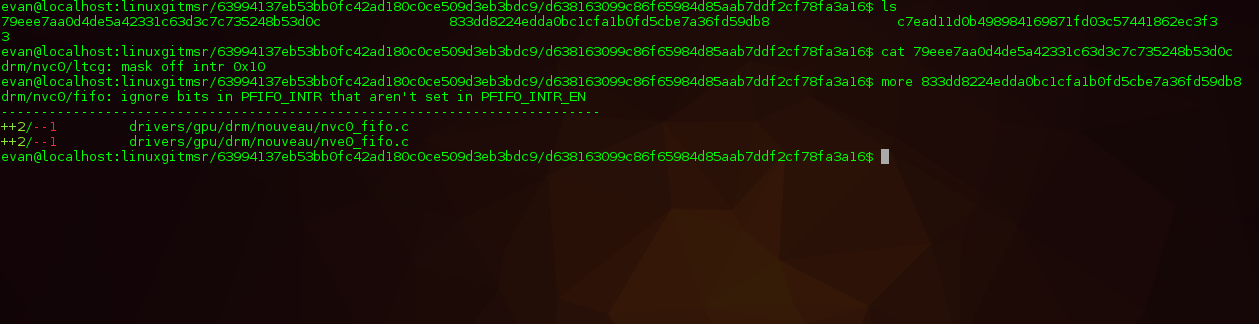
\includegraphics[width=0.47\textwidth]{figures/shell.png}
	\caption{Shell Design}
	\label{fig:shell}
\end{figure}

\evantodo{Put this in discussion section}
The main issue with this design is that a user will always move from the
top-down without any additional filtering. Furthermore, it presents the user
with the commit hashes, which provide no explanation of what the commit or
merge may contain.

\subsection{Web-based Tool}

There are multiple reasons for building the system into a web-based tool.
Putting the tool onto the web enables users to use the system without having to
install anything, making the system platform independent. A web-based tool can
utilize more interactive means of navigation, and provide a better explanation
of what each commit or merge may contain.

The web-based tool provides many mechanisms to enable users to better navigate
and understand changes in the kernel. These mechanisms include searching,
commit messages, files edited, modules edited, and two types of tree viewers.

\begin{figure}[h]
	\centering
	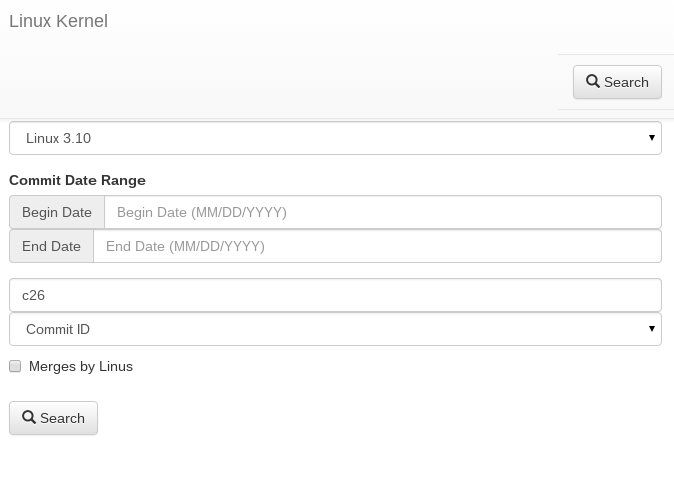
\includegraphics[width=0.47\textwidth]{figures/search.png}
	\caption{Search View}
	\label{fig:search}
\end{figure}

Searching allows a user to filter our commits and merges that are irrelevant.
The search mechanism breaks down the results by release version. A user can
further narrow down the search range using the commit date range. This commit
date refers to the date of the creation of the top-level merge. Commits and
merges that are returned may have a commit date beyond the given range if they
were merged to a top-level merge within the date range. A user may then provide
a search text, filtering on the author name, the commit id, or keyword from the
log. Any part of the author name may show up in the results, including
searching by email address. The commit ID must be specified from the first
character to the last character. For example, the commit
`c267548755a184ef97301071300c1739a564e135' is returned when the user searches
for a commit id of `c26' in the 3.10 Linux kernel.

\begin{figure}[h]
	\centering
	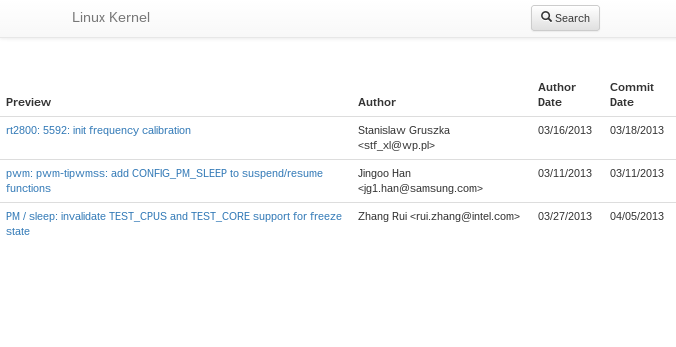
\includegraphics[width=0.47\textwidth]{figures/search_results.png}
	\caption{Search Results}
	\label{fig:results}
\end{figure}

In the search results , the user is presented with the one-line log message
preview, the author's name and email, the date the commit was authored, and the
date the commit was committed. \evantodo{a better definition for commit date}
The commit date and author date will usually be the same, however, if the
commit has been rebased, the commit date will be different than the authored
date, and will always be after the authored date. The first and third entries
in figure \ref{fig:results} have been rebased in the past. \evan{We are unable
to show the rebases.}

\begin{figure}[h]
	\centering
	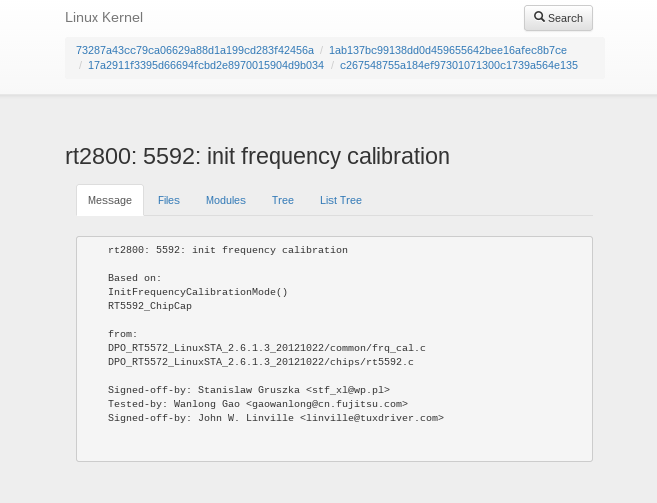
\includegraphics[width=0.47\textwidth]{figures/message_view.png}
	\caption{Commit Message}
	\label{fig:message}
\end{figure}

The first view displays the full commit log. From this, a user is able to see
hat they would see had they searched for the commit using git log. This doesn't
provide additional information to the other tools, but helps to complete the
functionality of the tool. This information provides a user with the
information about the content of the commit and who has looked over the commit
to ensure that it is good quality. The message for merges may also contain the
information about the commits that are being merged into a given merge. The
information within these messages is highly variable, and is completely
dependent on the author's style. As the user moves toward the top-level merge,
the quality of these messages generally improve.

\begin{figure}[h]
	\centering
	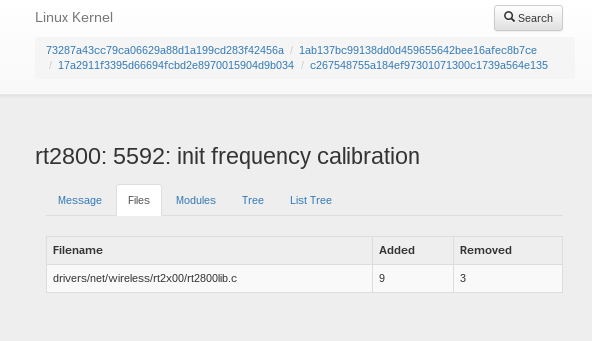
\includegraphics[width=0.47\textwidth]{figures/file_view.png}
	\caption{Commit Files}
	\label{fig:files}
\end{figure}

The second tab is the files tab. This tab provides information on what files
have been edited, how many lines were added, and how many lines were removed in
a given commit. This functionality is similar to the other tools available. Our
tree-based design model allows us to extend this functionality to merges, which
the other tools are unable to show. When a file is edited multiple times from
different commits within a merge, we simply add the added and removed lines to
the values already stored. \evan{At this time, we don't have a mechanism to
process the diff information to determine which lines were changed, and in what
order.}

\begin{figure}[h]
	\centering
	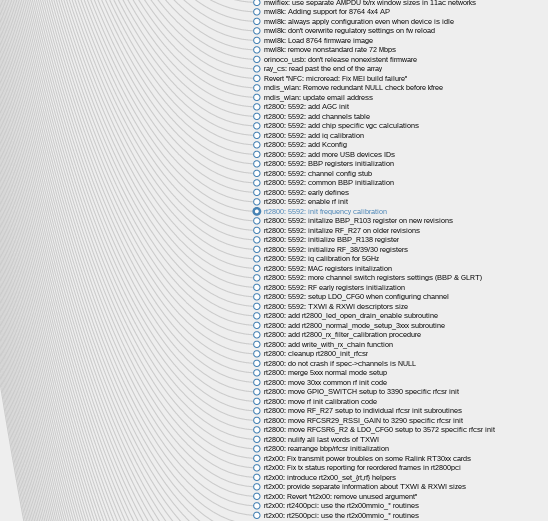
\includegraphics[width=0.47\textwidth]{figures/tree_view.png}
	\caption{Commit Tree View}
	\label{fig:files}
\end{figure}

The third tab shows the tree view. The tree view is what makes this tool unique
to the other tools. It provides a full view of the entire merge tree. It
originally centres at the current commit or merge, but allows a user to inspect
the other commits and merges surrounding it. A user may then navigate to any of
the commits by simply double-clicking on it.

\begin{figure}[h]
	\centering
	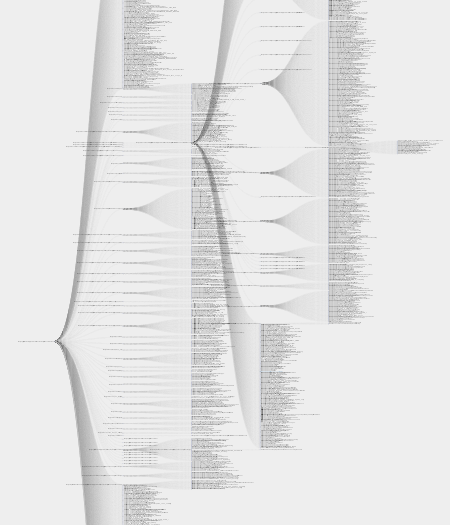
\includegraphics[width=0.47\textwidth]{figures/tree_zoom.png}
	\caption{Tree zoomed out}
	\label{fig:files}
\end{figure}

Some of the merge trees are very large, containing thousands of commits and
merges. Clicking on subtrees will cause them to minimize, only showing parts of
the tree that are of interest to the user. Furthermore, the user can zoom the
tree by scrolling the mouse wheel to see more of the topology of the tree, or
to see the details of a given part of the tree.

The last tab contains another type of tree view. This tree is in the form of
nested lists, and is designed to more closely model the tree hierarchy view of
file browsers. This tree only contains the commits and merges that are within
the subtrees of the current merge. A commit will never have any items in this
tab, as it is a leaf node, so it cannot contain subtrees. To accompany the
tree, we include breadcrumbs at the top. The last item in the breadcrumb list
is the current commit, the next item is the parent of the current commit, and
the first item is the top-level merge into the kernel.


\section{Future Work}
We have limited search functionality regarding actual files involved in
commits. If a user knows which file they are working with and what has changed
in a given file, they are unable to look specifically for commits pertaining to
that file. Adding a search filter for searching by file would allow maintainers
to perform this search.

Currently, there are still various features that have bad performance. More
work is required to get those features responding more quickly, or providing an
asynchronous mechanism and loading bars to improve user experience.

At this time, we have no evidence that our tool is able to improve the
work-flow of maintainers. We believe that the tool is able to improve the
work-flow and performance of maintainers because it is able to better assist
users because it provides cleaner mechanisms of working with the data. It is
able to provide more relevant information, while removing information that is
irrelevant to a given module or set of merges.

\end{document}
